\section{\textit{Simplification} de CFG}
\label{sec:simplification}

  % Program Slicing

  Le \textit{program slicing}, ou \textit{slicing}, est le calcul d'un
  ensemble d'instructions d'un programme qui affecte les valeurs des
  variables à un certain moment de l'exécution de celui-ci. Un
  \textit{slice} est donc un sous-ensemble d'instructions apartenant à
  l'ensemble des instructions du programme. Ce sous-ensemble
  d'instructions est tel qu'il possède un comportement équivalent au
  programme originial vis-à-vis de la valuation d'un sous-ensemble de
  variables du programme.

  Quand le \textit{slicing} s'applique à une seule procédure monolithique on
  parle de \textit{slicing} intraprocédural. En revanche lorsque le
  \textit{slicing} s'applique à un programme entier, au delà des frontières
  d'une procédure, on parle de \textit{slicing} interprocedural.

  \vspace{1em}

  % Intérêt du Program Slicing des CFG pour la vérification de modèle.

  Pour pallier au problème de l'explosion de l'espace d'état inhérent à la
  vérification des modèles il est nécessaire de réduire au maximum la quantité
  d'informations qui définit l'état du système. Le \textit{slicing} des CFG permet
  de ne conserver dans l'espace d'état du système uniquement les informations
  définissant l'état des variables -- registre ou contenu de la pile -- dont la
  valuation influt directement sur le flot de contrôle.

  Il n'est, en effet, pas nécessaire de conserver dans l'espace d'état du
  système les valuations de toutes les variables qui n'agissent pas directement
  sur le flot de contrôle puisqu'elles n'influent pas sur le temps d'exécution.
  
  \vspace{1em}
  
  % Program Slicing à base de graphes

  \begin{figure}[ht]
    \centering
    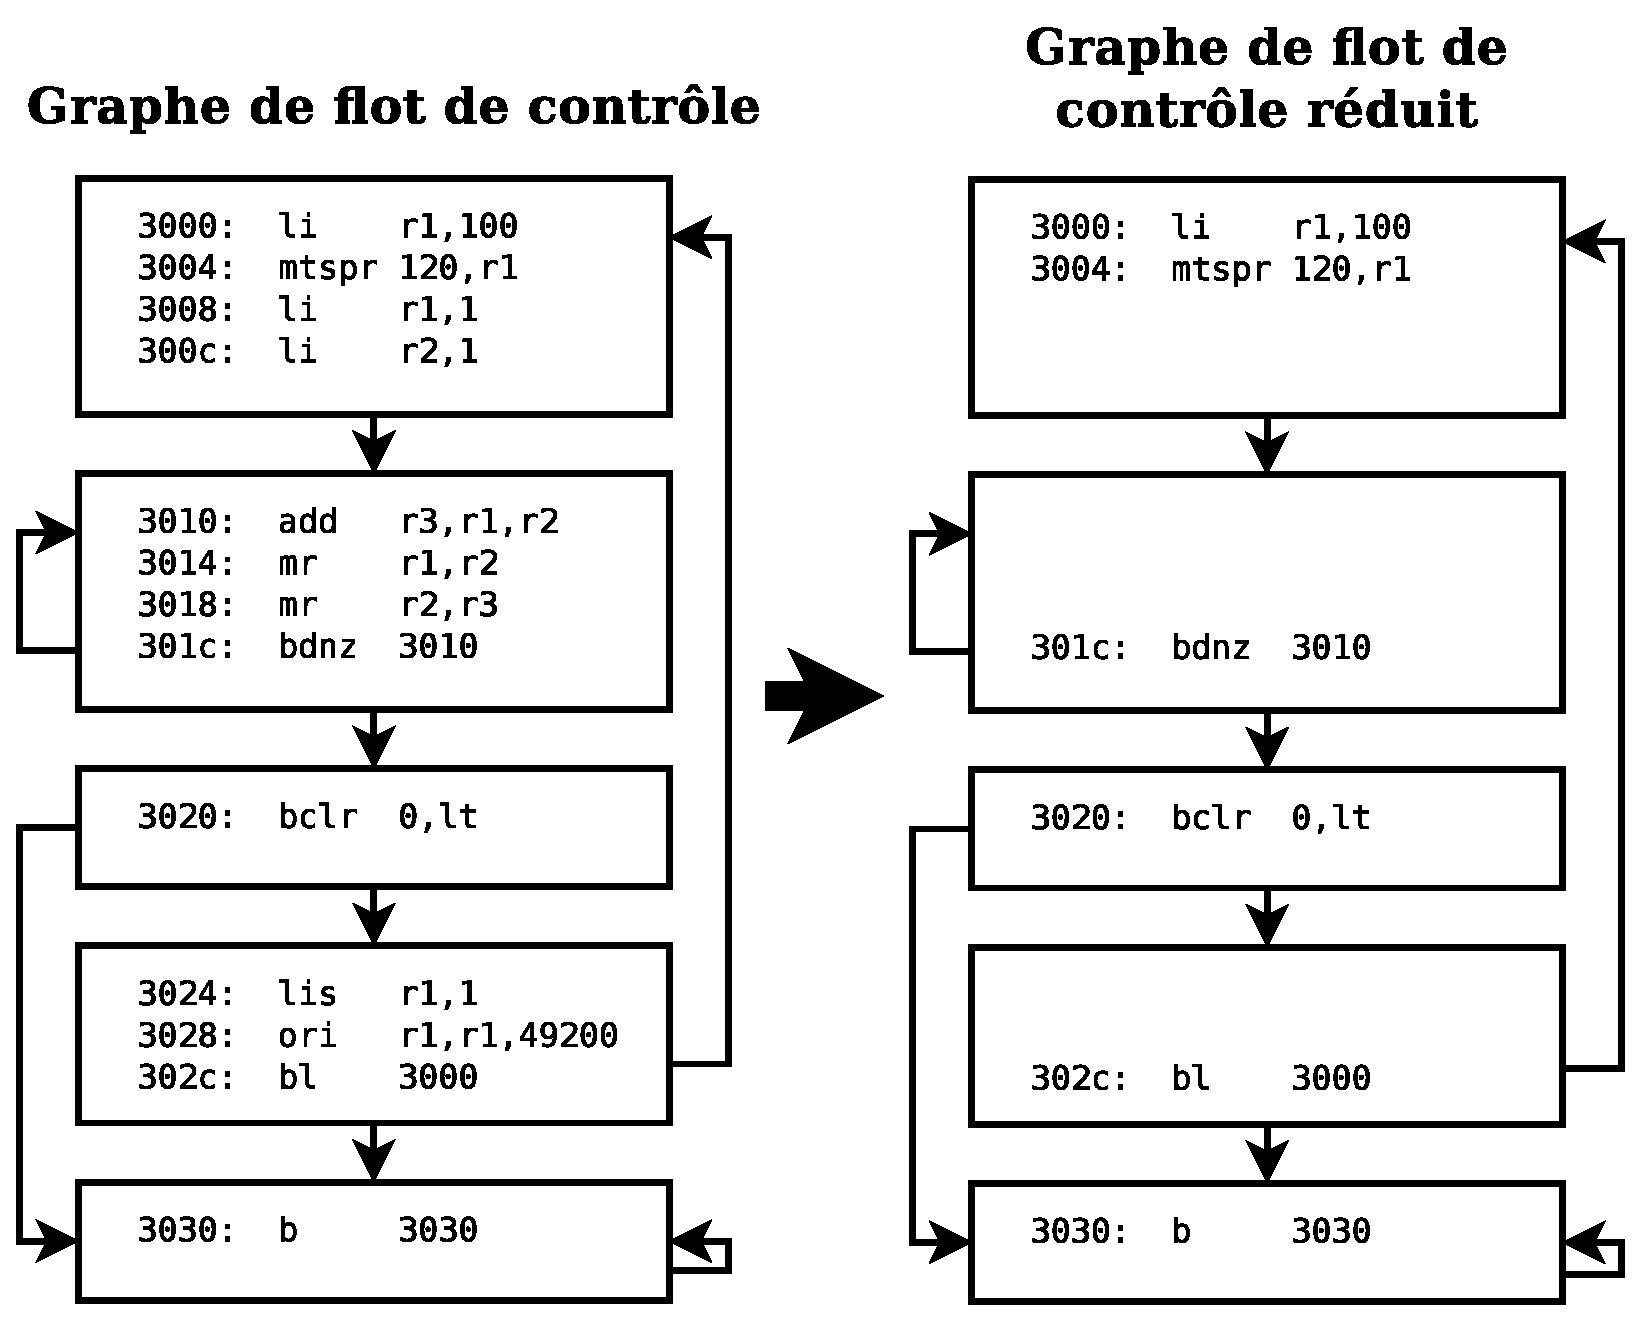
\includegraphics[scale=0.3]{img/slicing.eps}
    \caption{Processus de \textit{slicing} d'un CFG}
    \label{fig:slicing}
  \end{figure}
    
  Soit le CFG $G = (V, E, u, v)$. Un n{\oe}ud $d \in V$ domine
  (resp. post-domine) un n{\oe}ud $n \in V$ si et seulement si tous les chemins
  reliant $u$ (resp. $v$) et $n$ passent par $d$. Par définition, chaque
  n{\oe}ud se domine et post-domine lui-même. Un n{\oe}ud $d$ domine
  (resp. post-domine) strictement un n{\oe}ud $n$ si $d$ domine
  (resp. post-domine) $n$ et si $d$ n'est pas le n{\oe}ud $n$.

  Le dominateur (resp. post-dominateur) immédiat d'un n{\oe}ud $n$ est le
  n{\oe}ud qui domine (resp. post-domine) strictement $n$ mais qui ne domine
  (resp. post-domine) strictement aucun autre n{\oe}ud qui domine
  (resp. post-domine) strictement $n$. Tous les n{\oe}uds de $V$ ont un unique
  dominateur (resp. post-dominateur) immédiat excépté $u$ qui n'en a pas. Un
  arbre dominateur (resp. post-dominateur) est un graphe où l'ensemble des
  voisins d'un n{\oe}ud constitue l'ensemble des n{\oe}uds qu'il domine
  (resp. post-domine) immédiatement. Comme le dominateur (resp. post-dominateur)
  immédiat est unique, ce graphe est un arbre. Le n{\oe}ud d'entrée du CFG $u$
  est la racine de l'arbre.

  \vspace{1em}
  
  L'algorithme de \textit{slicing} implémenté s'appuie sur la méthode
  évoquée ci-après -- cf. \cite{CF97}. Les dépendances de données du
  programme y sont représentées par l'arbre post-dominateur et par des
  chaines de \textit{use-definition}. Ces chaines relient chaque
  utilisation d'une variable aux définitions qui peuvent l'affecter.

  Les dépendances de contrôle du programme sont manipulés à travers un graphe de
  dépendance de contrôle. Un graphe de dépendance de contrôle est un graphe où
  les arcs signifient un lien de dépendance entre la valuation du n{\oe}ud origine
  et l'exécution du n{\oe}ud cible.
